% Options for packages loaded elsewhere
\PassOptionsToPackage{unicode}{hyperref}
\PassOptionsToPackage{hyphens}{url}
%
\documentclass[
]{article}
\usepackage{amsmath,amssymb}
\usepackage{iftex}
\ifPDFTeX
  \usepackage[T1]{fontenc}
  \usepackage[utf8]{inputenc}
  \usepackage{textcomp} % provide euro and other symbols
\else % if luatex or xetex
  \usepackage{unicode-math} % this also loads fontspec
  \defaultfontfeatures{Scale=MatchLowercase}
  \defaultfontfeatures[\rmfamily]{Ligatures=TeX,Scale=1}
\fi
\usepackage{lmodern}
\ifPDFTeX\else
  % xetex/luatex font selection
\fi
% Use upquote if available, for straight quotes in verbatim environments
\IfFileExists{upquote.sty}{\usepackage{upquote}}{}
\IfFileExists{microtype.sty}{% use microtype if available
  \usepackage[]{microtype}
  \UseMicrotypeSet[protrusion]{basicmath} % disable protrusion for tt fonts
}{}
\makeatletter
\@ifundefined{KOMAClassName}{% if non-KOMA class
  \IfFileExists{parskip.sty}{%
    \usepackage{parskip}
  }{% else
    \setlength{\parindent}{0pt}
    \setlength{\parskip}{6pt plus 2pt minus 1pt}}
}{% if KOMA class
  \KOMAoptions{parskip=half}}
\makeatother
\usepackage{xcolor}
\usepackage[margin=1in]{geometry}
\usepackage{color}
\usepackage{fancyvrb}
\newcommand{\VerbBar}{|}
\newcommand{\VERB}{\Verb[commandchars=\\\{\}]}
\DefineVerbatimEnvironment{Highlighting}{Verbatim}{commandchars=\\\{\}}
% Add ',fontsize=\small' for more characters per line
\usepackage{framed}
\definecolor{shadecolor}{RGB}{248,248,248}
\newenvironment{Shaded}{\begin{snugshade}}{\end{snugshade}}
\newcommand{\AlertTok}[1]{\textcolor[rgb]{0.94,0.16,0.16}{#1}}
\newcommand{\AnnotationTok}[1]{\textcolor[rgb]{0.56,0.35,0.01}{\textbf{\textit{#1}}}}
\newcommand{\AttributeTok}[1]{\textcolor[rgb]{0.13,0.29,0.53}{#1}}
\newcommand{\BaseNTok}[1]{\textcolor[rgb]{0.00,0.00,0.81}{#1}}
\newcommand{\BuiltInTok}[1]{#1}
\newcommand{\CharTok}[1]{\textcolor[rgb]{0.31,0.60,0.02}{#1}}
\newcommand{\CommentTok}[1]{\textcolor[rgb]{0.56,0.35,0.01}{\textit{#1}}}
\newcommand{\CommentVarTok}[1]{\textcolor[rgb]{0.56,0.35,0.01}{\textbf{\textit{#1}}}}
\newcommand{\ConstantTok}[1]{\textcolor[rgb]{0.56,0.35,0.01}{#1}}
\newcommand{\ControlFlowTok}[1]{\textcolor[rgb]{0.13,0.29,0.53}{\textbf{#1}}}
\newcommand{\DataTypeTok}[1]{\textcolor[rgb]{0.13,0.29,0.53}{#1}}
\newcommand{\DecValTok}[1]{\textcolor[rgb]{0.00,0.00,0.81}{#1}}
\newcommand{\DocumentationTok}[1]{\textcolor[rgb]{0.56,0.35,0.01}{\textbf{\textit{#1}}}}
\newcommand{\ErrorTok}[1]{\textcolor[rgb]{0.64,0.00,0.00}{\textbf{#1}}}
\newcommand{\ExtensionTok}[1]{#1}
\newcommand{\FloatTok}[1]{\textcolor[rgb]{0.00,0.00,0.81}{#1}}
\newcommand{\FunctionTok}[1]{\textcolor[rgb]{0.13,0.29,0.53}{\textbf{#1}}}
\newcommand{\ImportTok}[1]{#1}
\newcommand{\InformationTok}[1]{\textcolor[rgb]{0.56,0.35,0.01}{\textbf{\textit{#1}}}}
\newcommand{\KeywordTok}[1]{\textcolor[rgb]{0.13,0.29,0.53}{\textbf{#1}}}
\newcommand{\NormalTok}[1]{#1}
\newcommand{\OperatorTok}[1]{\textcolor[rgb]{0.81,0.36,0.00}{\textbf{#1}}}
\newcommand{\OtherTok}[1]{\textcolor[rgb]{0.56,0.35,0.01}{#1}}
\newcommand{\PreprocessorTok}[1]{\textcolor[rgb]{0.56,0.35,0.01}{\textit{#1}}}
\newcommand{\RegionMarkerTok}[1]{#1}
\newcommand{\SpecialCharTok}[1]{\textcolor[rgb]{0.81,0.36,0.00}{\textbf{#1}}}
\newcommand{\SpecialStringTok}[1]{\textcolor[rgb]{0.31,0.60,0.02}{#1}}
\newcommand{\StringTok}[1]{\textcolor[rgb]{0.31,0.60,0.02}{#1}}
\newcommand{\VariableTok}[1]{\textcolor[rgb]{0.00,0.00,0.00}{#1}}
\newcommand{\VerbatimStringTok}[1]{\textcolor[rgb]{0.31,0.60,0.02}{#1}}
\newcommand{\WarningTok}[1]{\textcolor[rgb]{0.56,0.35,0.01}{\textbf{\textit{#1}}}}
\usepackage{graphicx}
\makeatletter
\def\maxwidth{\ifdim\Gin@nat@width>\linewidth\linewidth\else\Gin@nat@width\fi}
\def\maxheight{\ifdim\Gin@nat@height>\textheight\textheight\else\Gin@nat@height\fi}
\makeatother
% Scale images if necessary, so that they will not overflow the page
% margins by default, and it is still possible to overwrite the defaults
% using explicit options in \includegraphics[width, height, ...]{}
\setkeys{Gin}{width=\maxwidth,height=\maxheight,keepaspectratio}
% Set default figure placement to htbp
\makeatletter
\def\fps@figure{htbp}
\makeatother
\setlength{\emergencystretch}{3em} % prevent overfull lines
\providecommand{\tightlist}{%
  \setlength{\itemsep}{0pt}\setlength{\parskip}{0pt}}
\setcounter{secnumdepth}{-\maxdimen} % remove section numbering
\ifLuaTeX
  \usepackage{selnolig}  % disable illegal ligatures
\fi
\IfFileExists{bookmark.sty}{\usepackage{bookmark}}{\usepackage{hyperref}}
\IfFileExists{xurl.sty}{\usepackage{xurl}}{} % add URL line breaks if available
\urlstyle{same}
\hypersetup{
  pdftitle={DSCI445 - Homework 4},
  pdfauthor={Your Name},
  hidelinks,
  pdfcreator={LaTeX via pandoc}}

\title{DSCI445 - Homework 4}
\author{Your Name}
\date{}

\begin{document}
\maketitle

Be sure to \texttt{set.seed(445)} at the beginning of your homework.

\begin{Shaded}
\begin{Highlighting}[]
\CommentTok{\#reproducibility}
\FunctionTok{set.seed}\NormalTok{(}\DecValTok{445}\NormalTok{)}
\end{Highlighting}
\end{Shaded}

\begin{enumerate}
\def\labelenumi{\arabic{enumi}.}
\item
  In this exercise, we will generate simulated data, and then use this
  data to perform best subset selection.

  \begin{enumerate}
  \def\labelenumii{\alph{enumii})}
  \item
    Use \texttt{rnorm} to generate a predictor \(X\) of length
    \(n = 100\) and a noise vector \(\epsilon\) also f length
    \(n = 100\).
  \item
    Generate a response vector \(Y\) of length \(n = 100\) according to
    the model \[
     Y = \beta_0 + \beta_1 X + \beta_2 X^2 + \beta_3 X^3 + \epsilon
     \] where
    \(\beta_0 = 1, \beta_1 = -0.5, \beta_2 = 2, \beta_3 = -1\).
  \item
    Use the \texttt{regsubsets} function in the \texttt{leap} package to
    perform best subset selection in order to choose the best model
    containing the predictors \(X, X^2, \dots, X^{10}\). What is the
    best model obtained according to \(C_p\), BIC, and Adjusted \(R^2\)?
    Shoe some plots to provide evidence for your answer and report the
    coefficients of the best model obtained.

    {[}\textbf{Hint 1:} The \texttt{poly} function may be useful for
    creating the model formula.{]}

    {[}\textbf{Hint 2:} You will need to make a data frame with your X
    and Y variables.{]}
  \item
    Repeat c.~using forward stepwise selection and also using backwards
    stepwise selection. How does your answer compare to the results in
    c.?
  \item
    Now fit a lasso model to the simulated data using
    \(X, X^2, \dots, X^{10}\) as predictors. Use \(10\)-fold CV to
    choose the optimal value of \(\lambda\). Create plots of the CV
    error as a function of \lambda. Report the resulting coefficient
    estimates and discuss the results obtained.
  \end{enumerate}
\item
  In this exercise we will predict the number of applications received
  using the other variables in the \texttt{College} data set (in the
  \texttt{ISLR} package).

  \begin{enumerate}
  \def\labelenumii{\alph{enumii})}
  \item
    Split the data into training (60\%) and ``test'' (40\%) set
    randomly.
  \item
    Fit a linear model using least squares on the training set and
    report the test set error obtained.
  \item
    Fit a ridge regression model on the training set with \(\lambda\)
    chosen using 10-fold CV (on the training set only). Report the test
    error obtained.
  \item
    Fit the lasso on the training set with \(\lambda\) chosen using
    10-fold CV (on the training set only). Report the test error
    obtained, along with the number of non-zero coefficient estimates.
  \item
    Fit a PCR model on the training set with \(M\) chosen using 10-fold
    CV (on the training set only). Report the test error obtained, along
    with the value of \(M\) selected by CV.
  \item
    Fit a PLS model on the training set with \(M\) chosen using 10-fold
    CV (on the training set only). Report the test error obtained, along
    with the value of \(M\) selected by CV.
  \item
    Comment on the results obtained. How acurately can we predict the
    number of college applications received? Is there much difference
    among the test errors resulting from these five approaches?
  \end{enumerate}
\item
  We have seen that as the number of features used in a model increases,
  the training error will necessarily decrease, but the test error may
  not. We will explore this with a simulated data set. Run the following
  code to generate your dataset.

\begin{Shaded}
\begin{Highlighting}[]
\NormalTok{p }\OtherTok{\textless{}{-}} \DecValTok{20}
\NormalTok{n }\OtherTok{\textless{}{-}} \DecValTok{1000}

\NormalTok{X }\OtherTok{\textless{}{-}} \FunctionTok{matrix}\NormalTok{(}\FunctionTok{rnorm}\NormalTok{(n }\SpecialCharTok{*}\NormalTok{ p), }\AttributeTok{nrow =}\NormalTok{ n, }\AttributeTok{ncol =}\NormalTok{ p) }\DocumentationTok{\#\# predictors}
\NormalTok{beta }\OtherTok{\textless{}{-}} \FunctionTok{matrix}\NormalTok{(}\FunctionTok{c}\NormalTok{(}\FunctionTok{rnorm}\NormalTok{(}\DecValTok{8}\NormalTok{), }\FunctionTok{rep}\NormalTok{(}\DecValTok{0}\NormalTok{, p }\SpecialCharTok{{-}} \DecValTok{8}\NormalTok{)), }\AttributeTok{ncol =} \DecValTok{1}\NormalTok{) }\DocumentationTok{\#\# 12 elements are equal to zero}

\NormalTok{y }\OtherTok{\textless{}{-}}\NormalTok{ X }\SpecialCharTok{\%*\%}\NormalTok{ beta }\SpecialCharTok{+} \FunctionTok{rnorm}\NormalTok{(n, }\DecValTok{0}\NormalTok{, .}\DecValTok{5}\NormalTok{) }\DocumentationTok{\#\# y = Xbeta + epsilon}
\end{Highlighting}
\end{Shaded}

  \begin{enumerate}
  \def\labelenumii{\alph{enumii}.}
  \item
    Split your data into a training set containing 100 observations and
    a test set containting 900 observations.
  \item
    Perform best subset selection on the training set and plot the
    training set MSE associated with the best model of each size
    (\textbf{Hint} How do we calculate MSE?).
  \item
    Plot the test set MSE associated with the best model of each size.
    Hint, to get the predicted values, use matrix multiplication
    (\texttt{\%*\%}) to multiply the test data by the fitted
    coefficients of each model: \(X\hat{\beta}\). Note there is no
    \texttt{predict} function for \texttt{regsubsets} objects.
  \item
    For which model size does the test set MSE take its minimum value?
    Comment on your results.
  \item
    How does the model at which the test set MSE is minimized compare to
    the true model used to generate the data? Comment on the coefficient
    values.
  \end{enumerate}
\item
  We will now try to predict per capita crime rate in the
  \texttt{Boston} data set from the \texttt{ISLR} package.

  \begin{enumerate}
  \def\labelenumii{\alph{enumii}.}
  \item
    Try out some of the regression methods explored in this chapter such
    as best subset, the lasso, ridge regression, and PCR. Present and
    discuss results for the approaches that you consider.
  \item
    Propose a model or a set of models that seem to perform well on this
    data set and justify your answer. Make sure that you are evaluating
    performance using validation error, cross-validation error, or some
    other reasonable alternative (not just training error).
  \item
    Does your chosen model involve all of the features in the data set?
    Why or why not?
  \end{enumerate}
\end{enumerate}

Turn in in a pdf of your homework to canvas using the provided Rmd file
as a template. Your Rmd file on the server will also be used in grading,
so be sure they are identical.

\textbf{Be sure to share your server project with the instructor and
grader. You only need to do this once per semester.}

\begin{enumerate}
\def\labelenumi{\arabic{enumi}.}
\item
  Open your \texttt{homeworks} project on liberator.stat.colostate.edu
\item
  Click the drop down on the project (top right side) \textgreater{}
  Share Project\ldots{}

  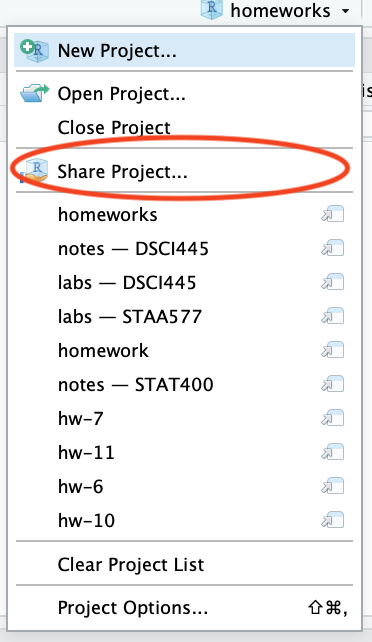
\includegraphics[width=0.25\linewidth]{share_project}
\item
  Click the drop down and add ``dsci445instructors'' to your project.

  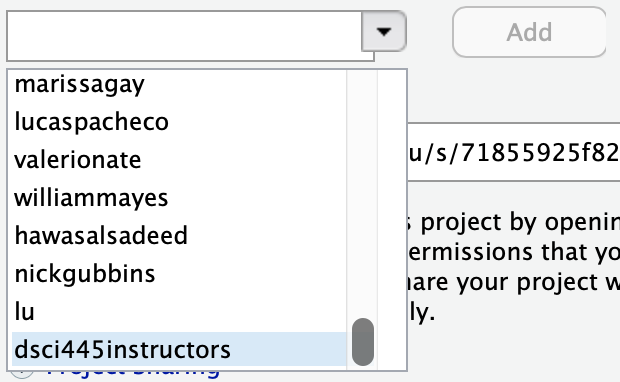
\includegraphics[width=0.25\linewidth]{share_dropdown}
\end{enumerate}

This is how you \textbf{receive points} for reproducibility on your
homework!

\end{document}
